\chapter{Bubble Interactions 80\%}
\section{Introduction}

Acoustic sources will, in general, interact with one another. %, with this interaction  mediated by sound.
%The study of vortex-vortex interactions has a  long history  \cite{Whittaker1951},
The study of the interactions between pulsating bodies
is of  interest in medical ultrasound because pulsating micron sized bubbles are used as contrast agents.
The induced motion  between neighbouring bubbles has been photographed
and the force between them is often  modelled according to Bjerknes' law  \cite{Crum1971}.
This states that the average force on a bubble, $\scalar{f}$, is
equal to volume displaced by the bubble, $ V$, multiplied the acceleration 
induced by a pressure gradient, $\vdel p$ \cite{Bjerknes1905,Crum1971, Leighton1990},
\begin{align}
  \label{eqn:Bjerknes}
  \scalar{f} = \scalar{V(t)\vdel p(\vx, t)}.
\end{align}
The  average force  over an oscillation cycle will not be zero if the bubble do not pulsate in phase with the sound wave.
% f the oscillations arThe phase is denoted with a 
% % and the pressure oscillates sinusoidally with a frequency $\omega$, so that  $P(\vx, t) = P(\vx)\sin\lr{\omega t}$.
% To see that the average can give non-zero results,
If we assume that the spatial and temporal components of the pressure may be separated, 
 so that  $P(\vx, t) = P(\vx)\sin\lr{\omega t}$,
 and assume that the bubble's pulsations are small, 
 so that $V(t) = V_0\sin\lr{\omega t + \beta}$,
then 
$\beta$ is the phase of the bubble's oscillations in comparison to the driving sound wave.
%Then 
%\begin{align}
%  \scalar{F} = V_0\vdel P(\vx) \scalar{\sin(\omega t+\beta)\sin(\omega t)} =  \frac{1}{2}V_0\vdel P(\vx) \cos(\beta)
%\end{align}
The resultant force over a cycle of oscillation is 
 $\scalar{F} = \frac{1}{2}V_0\vdel P(\vx) \cos(\beta)$.
%The strength of the force is determined by $\cos(\beta)$,
%which can be either positive or negative.

The  cost of this simple model is that the equations describing the surrounding fluid are linearised.
Vorticity is not considered and we are entirely removed from the general problem of 
turbulence-sound interaction.
This is a shame, for while it is true that the acoustic output of a pulsating bubble far exceeds that of turbulent sources,
turbulence is still excepted to have an influence on the bubble's motion.
%Bubbles will not only be carried by turbulent flow but will also interact with the sound generated by it.

Bjerknes' law, in itself, assumes little about the bubble. 
It requires only a pulsating volume.
The details of the bubble, such as its surface tension, are hidden in the parameter $\beta$ that specifies how close to resonance the bubble is \cite{Leighton1990}.
The motion and interaction of a bubble, therefore, 
can be firmly set within the context of turbulence-sound interactions, 
so long as the bubbles mass varies when the bubble interacts with an acoustic field.
This chimes with the attempts to use Hicks'  spherical vortex as a model of a bubble \cite{Levine1959}.
Indeed, so long as the bubble is small compared 
to the wavelength of the sound with which it interacts, then any vortex should do.
%Bjerknes' law not require us to be too specific.


In this report, as a means of investigating the interactions between bubbles and sound in its full context,
models to describe sound-turbulence interactions in general are suggested.
To simplify the approach we consider only the special case of when the interactions are measured acoustically,
such as is the case when the turbulence is measured with ultrasound.
%The formulation therefore remains general, 
It turns out that  acoustics  is greatly simplified when imaged with sound.
In fact,
as is shown in \secref{measurement},
 Lighthill's formulation of acoustics reduces to an {\em exact} analogue of electromagnetism.
The reasons for this are briefly discussed in \secref{measurement} 
and in more detail in a companion paper elsewhere in these proceedings.

To find the physical consequences of the equivalence,
the analogy is used to define an acoustic Lagrangian.
%The exactness of the analogy has a number of consequences.
%To find them, it is noted that since the field equations are the same, 
%the acoustic field and the electromagnetic field 
%can be characterised by a common Lagrangian.
This is done in \secref{lagrangian} and the implications to angular momentum and helicity are discussed.

Starting from the Lagrangian, the acoustic energy momentum tensor follows,
from which the required interaction laws between sound and turbulence can be found.
Unsurprisingly, in light of the analogy found, 
this is the Lorentz force law  (\secref{spinless}).

Swirl, which is  the motion along a vortex ring, for example, is harder to incorporate.
This is because, as argued in \secref{spin}, a vortex with swirl has an intrinsic angular momentum
which will be involved in the interaction.
To simplify, the size of the vortex is reduced to a point.
Its swirl and velocity can then be modelled with a co-moving frame of reference,
%One axis of the coordinate frame traces the path of the vortex,
%another traces the rotion.
%The helical path through spacetime of any given particle within the vortex can then be traced.
%This is discussed in \secref{spin}.  
The interaction term $\beta$ is included in \secref{bubble},  enabling bubble motion to be modelled.
The model chosen has a great deal of common with classical models of quantum  spin.
Our thinking has been particularly influenced by David Hestenes' timelike  Zitterbegung model of the election \cite{Hestenes1973, Hestenes1990, HestenesResearchProgram}.  
It is interesting how naturally the zitterbewegung model can be applied to turbulence.

Finally, we note that the geometric nature of the models discussed is most straightforward
and  concise when expressed in the {\em Spacetime Algebra} of David Hestenes \cite{Hestenes2003}.
%This notation is sufficiently close to usual 3-dimensional vector algebra to be familiar,
%but unfortunately space here does not permit an introduction to the algebra.
Important results will be projected into the laboratory frame,
so that they can be understood entirely with familiar 3-dimensional vector algebra.
We use the convention that three dimensional vectors are displayed in bold.
This helps to distinguish them from their spacetime analogues.







 

%Sir James Lighthill, in his formulation of acoustics \cite{Lighthill1952},
%gave a general framework for calculating the sound generated by turbulence with a minimum of approximation.


%The influence of boundaries was added to the formulation by Curle \cite{Curle1955} and Ffowcs Williams and Hawkings \cite{FfowcsWilliams1969}.
%More recently,  formulations in terms of the vorticity and enthalpy have also proven useful \cite{Howe1998}.
%Development has been rapid, and this must be due, in no small part, to the common point of departure enabled by Lighthill.
%The relation of special cases to the whole is clear, it is easy to see the wood from the trees.
% The turbulent sources in Lighthill's theory will in general interact with each other.
% There is a long history in studying the interactions of vorticies \cite{Whittaker1951}, 
% but yet no 
% where the force between the rings `acts at a distance', and  propagates through the medium via sound waves.
% The vorticity formulation of Lighthill's equation, therefore,
% seems ideally placed to formulate sound-acoustic source dynamics in a general way.
% This is a difficult problem in general,
% but a simple solution is possible when the interaction is measured by ultrasound,
% and is outlined in \secref{Lorentz}.
% It turns out that ultrasound is simpler than acoustics in general due to the way in which ultrasound defines time and space.
% This is discussed more in \secref{Measurement}.

% In medical ultrasound, however, the interaction of purely turbulent sources of sound are not of primary interest.
% Rather, focus is directed at the  interactions between  micron-sized pulsating bubbles that are used as contrast agents.
% Usually, when modelling such interactions the fluid is linearised early \cite{Crum1974,Leighton1990, Mettin1997},
% and so any effect of vorticity and turbulence is ignored$rho.
% This is unsatisfactory for two reasons.
% \nlist{
% \item Although the pulsating bubble is likely to dominate the sound generated in a region of turbulence,
%   it does not necessarily follow that the {\em motion } of the bubble is independent of the vorticity in the surrounding fluid.
% \item By linearising the fluid the general framework for sound-acoustic source interactions is being abandoned.
% }
% The first of these problems is the greater when it comes to predicating the results of an experiment.
% However, the second is the more grave.
% By approximating too early the theory becomes separated from the general theory of sound-source interaction, and progress becomes slow.
% Indeed, the Bjerknes force law that is often used to describe the interactions of bubbles has changed little since it was written down in 1905 \cite{Bjerknes1905},
% and this is not because it is without  problems.

% In this report we attempt to bring the description of the motion of a bubble within the Lighthill framework for ultrasonics outlined in \secref{Lorentz}.
% This is attempted in \secref{Zitter}.






%\section{Acoustically measured physics}\label{sec:measurement}

%Ultrasound measures both the spatial and temporal locations of an object from the time
%it takes a pulse of sound to propagate from a transducer and then to return again.
%If the sound is emitted  at a time $\tm$ and the sound returns at a time  $\tp$,
%then the temporal label $\tau(x)$ and the spatial label $\rho(x)$  for the object at the spacetime point $x$ is defined to be
%\sub{
%\label{eqn:radar}
%\begin{align}
% \tau(x) &= \frac{\tm + \tp}{2}, &&\text{and}& \rho(x) &= \frac{\tp - \tm}{2}c
%\end{align}
%}
%where $c$ is the speed of sound.
%It is noted, firstly, that equations \eqnref{radar} provide no method for determining the spatio-temporal location of an object absolutely,
%there is no preferred direction or location.
%Secondly the sound speed is a constant of the medium and so is independent of the motion of the transducer.

%It is  interesting to note that equations \eqnref{radar} are identical  to the `radar' definitions that Einstein used to define time and space \cite{Dolby2001},
%except that sound is used as the propagating signal rather than light.
%Likewise, Einsteins postulates also hold (as discussed in more detail in a companion paper elsewhere in these proceedings).
%Ultrasound is, therefore, a relativistic theory where the speed of sound takes the role of the speed of light.

%Lorentz invariant theories obey the measurement process of equation \eqnref{radar}
%and so form an appropriate point to begin the acoustically observed description of the medium.
%Here we assume that the medium is an ideal and homentropic fluid.
%In this case the speed of sound is $c^2 = \frac{\d p}{\d \epsillon}$
%where $\epsilon$ is the energy density and $p$ is the pressure.
%Natural units are chosen so that the speed of sound, which will shortly be set to equal the speed of light, is unity.
%From the definition of the sound speed we see that  the equation of state, $\epsilon \equiv \epsilon(p) = p$,
%enforces the speed speed condition.
%The equation  $p^{1/2} = \rho$ follows from the homentropy condition.
%These equations of state are the relativistic analogues to incompressibility and are  reviewed by  Taub \cite{Taub1978}.

%The 4-vector $A$ is defined to have the temporal and spatial components 
%\begin{align}
%  \phi &\equiv \gamma \frac{\epsilon + p}{\rho} = \gamma\lr{c^2 + h}, &&\text{and}&\vA &\equiv\phi \vv 
%\end{align}
%where  $\gamma = \frac{1}{\sqrt{1-\vv^2}}$ is the Lorentz factor and $h$ is the enthalpy.
%It is apparent that $\phi$ reduces to the total enthalpy $H = h+ \frac{v^2}{2}$ in the non-relativistic limit.
%Applying these conditions for acoustic measurement,
%the energy momentum tensor for a relativistic ideal fluid simplifies to
%\eqa{
%  T(a) = (\epsilon + p) a \cdot v v - a p =  \frac{1}{4}  A a A. 
%}
%In the absence of external forces the equations of motion, when expressed in the lab frame, are
%\eqal{
%   \vdel \cdot \vA &=  - \dt \phi  &&\text{and}& \dt \vA - \vv \times \lr{\vdel \times \vA}  + \vdel \phi &= 0.
%}{ContsRel}
%These are the acoustically measured versions of the continuity equation and the Euler's equation.

%By differentiating the continuity equation with respect to time
%and subtracting from the spatial derivative of Euler's equation, 
%a wave equation for the specific total enthalpy is obtained
%\subl{
%\eqa{
%   \lr{\vdel^2 - \dt^2}\phi
%  & = \vdel \cdot \lr{\vv \times\lr{\vdel \times \vA} } \equiv - \rho_q.
%\label{eqn:WavePhi}
%  \intertext{Alternatively, 
%    by differentiating the continuity equation with respect to space 
%    and adding it to the temporal derivative of Euler's equation,
%    a wave equation for $\vA$ is obtained,
%    }
%   \lr{\vdel^2 - \dt^2}\vA 
%   &  = - \vdel\times\lr{\vdel \times \vA} - \dt \lr{ \vv \times \lr{\vdel \times \vA}} \equiv -\vJ.
%    \label{eqn:WavevA}
%  }
%}{Waves}
%The right hand side of \eqnref{WavePhi} and  \eqnref{WavevA} have been interpreted as an acoustic source density and acoustic current density, respectively.
%Notice the nice property that the current is conserved $\vdel\cdot \vJ + \dt \rho_q = 0$.
%This pair of equations are the acoustically measured version of Lighthill's equations expressed in terms of enthalpy and vorticity \cite{Howe1998}.

%We complete this section by defining the Coriolis acceleration, $\vE = - \vv \times \lr{ \vdel \times \vA}$ and the vorticity $\vB = \vdel \times \vA$.
%Then \eqnref{Waves} are seen to be equivalent to Maxwell's equations in the Lorenz gauge ($\vdel \cdot \vA + \dt \phi = 0$).
%$\vA$ is interpreted as the analogue vector potential, $\phi$ the analogue scalar potential, $\vE$ the analogue electric field, and $\vB$ the analogue magnetic field.
%It is easy to confirm,
%\subl{
%\eqa{
%  \vdel \cdot \vE  &= q, %&& \text{from \eqnref{qdefn} and \eqnref{vELamb},} \label{eqn:M1} \\
%&  \vdel \times \vE &= -\dt  \vB, \label{eqn:ME} \\%&& \text{from  \eqnref{vELambPots} and \eqnref{IvBVort},} \label{eqn:M2} \\
%  \vdel \cdot \vB  &= 0, %\text{from \eqnref{IvBVort},}  \label{eqn:M3}\\
%&  \vdel \times \vB &=  \lr{ \vJ +\dt \vE}.%
%  %&& \text{from \eqnref{vJdefn} and \eqnref{IvBVort}.} \label{eqn:M4}
%}
%}{Maxwell}
%For example, the second of \eqnref{ME} is the vorticity equation. %, as confirmed by taking the curl of the second of \eqnref{ContsRel}
%By combing the acoustic source density  and the acoustic current into a single 4-vector $J$,
%equations \eqnref{Maxwell} can be combined into a single equation \cite{Doran2003}
%\eqal{
%  \del F = J
%}{MaxwellGA}
%where $F = \del \wedge A$ is the 4-vorticity.
%The acoustic field is therefore characterised by a single, linear equation.

%%When the turbulence  is confined to a bounded volume it is reasonable to call the region a particle.
%%Surfaces with an outward $\vE$-field (and therefore charge) are called Lamb surfaces.
%%Topologically, a toroid seem a favoured configuration \cite{}.

\section{Interactions of sound and turbulence}
%Usually, when imagining the average motion of particles in a sound wave,
%we think of the particles oscillating back and forth as the pressure perturbation passes through.
%This is because we think of sound waves as being longitudinal.

In \chapref{acousticSR} it was found that when measuring the world with sound,
the world should be described relativistically with reference to the speed of sound.
It was also found that the a sound wave, in this measurement system, obeys an exact analogue of
Maxwell's equations of electromagnetism.
That is, 
\sub{
\eqa{
  \vdel \cdot \vE &= \frac{\rho_q}{\permitivity},\tag{\ref{eqn:M1}}  \\ 
 \vdel \times \vB &= \permeability \vJ + \tfrac{1}{c^2} \dt E, \tag{\ref{eqn:M2}}\\
 \vdel \times \vE &= -\dt\vB\tag{\ref{eqn:M3}},\\
 \vdel \cdot \vB &= 0\tag{\ref{eqn:M4}}.
}
%\tag{\ref{eqn:M}}
}
where  $\vE$ is known as the Lamb vector and $\vB$ is the spatial vorticity.


Equations \eqnref{M1}-\eqnref{M4} imply that a sound waves can be considered to be a self-inducing vorticity-Coriolis wave.
The transverse nature (with respect to the direction of propagation)  of electromagnetic waves is well known, and applies equally to the vorticity and Coriolis fields here.
In this section we consider the implications of this observation.




\subsection{The acoustic Lagrangian}\label{sec:lagrangian}
%From equations \eqnref{Maxwell} acoustic sources are described by the same equations that characterise electromagnetic sources.
The common mathematical  description of acoustics and electromagnetism will result if both are derived from same Lagrangian,
%\begin{align}
 $ \L = \frac{1}{2} F \cdot F  - A \cdot J$.
%\end{align}
In the absence of sources ($J = 0$),
the canonical energy-momentum tensor, which expresses invariance with respect to translations,
is found to be \cite{Lasenby1993, Doran2003},  $T(a) = \lr{a\cdot \del A}\cdot F - \half a F \cdot F.$
The explicit dependence on $A$ can be moved to the bounding surface \cite{Lasenby1993}
to leave a manifestly gauge invariant form within the volume,
\begin{align}
\label{eqn:TAEM}
  \Tgi(a) = -\half F a F.
\end{align}
Similarly, the  adjoint to the canonical angular momentum of the acoustic field, which expresses the isometry of the acoustic medium, 
is found from the Lagrangian to be \cite{Lasenby1993}
\begin{align}
  \label{eqn:AM}
  \J(n) = T(n) \wedge x - A \wedge \lr{F\cdot n} = T(n) \wedge x - S(n).
\end{align}
The term $T(n) \wedge x$ is the  orbital angular momentum and $S(n)$ is the spin of the acoustic field.
The spin term is often suppressed by putting its influence in the boundary conditions,
but since we are interested in acoustic plain waves we shall not do this.
%This has the advantage of making the angular momentum manifestly gauge-invariant,
%although at the cost of making plain-waves (that reach to infinity) more inconvenient to handle.
%Again this isn't manifestly gauge invariant.
%When the fields diminish rapidly at infinity the angular momentum may be  expressed in gauge invarent form,
%the spin is absorbed into the angular momentum $T(n)$.
%However, such a procedure is not valid for plain wave solutions (as the field does not vanish at infinity)
% so we keep \eqnref{AM}.
%The spin in the lab frame  is
%\begin{align}
%  S(v) =A \wedge   \lr{F \wedge \gamma} = -\multi{\phi + \vA \vE}_2 = \phi phi I \vB_v 
 %  S(n) = A \cdot  \lr{F\wedge  n} =  \lr{A\cdot F} \wedge n %= -\phi I\vB
%\end{align}
%The spin in the lab frame  is
%\begin{align}
%  S(\g) =A \wedge   \lr{F \cdot \g} = -\phi \vE - I \vA \times \vE  = 
% %  S(n) = A \cdot  \lr{F\wedge  n} =  \lr{A\cdot F} \wedge n %= -\phi I\vB
%\end{align}

\subsection{Interpreting the transversivity of the sound pulse} \label{sec:transversivity}


An acoustic plain wave is  a  perturbation of the fluid particles in the direction of propagation of the pulse.
It is also a transverse wave in terms of the Coriolis and vorticity fields.
We now propose a method of squaring these seemingly contradictory views.

We consider a segment of the plain wave to be a narrow tube,
so that the entire plain wave is formed by adding together many such tubes.
Within the tube a pertabation in pressure propagates the sound wave longitudinally.
Outside of the tube no such pertabation exists.

Both within and outside of the tube  there is no vorticity and so there is no propagation of the transverse wave.
On the interface of the tube, however, there is shearing of the fluid:
the molecules  within tube move as the wave passes, the molecules outside do not.
This shearing induces a {\em vortex sheet} on the interface \cite{Howe1998}.
The vorticity is confined to the sheet 
and has a strength equal to the average speed of the molecules on either side of the interface.
From the acoustic analogue Maxwell's equations, this vorticity then induces a Coriolis acceleration orthogonal to the interface.
A longitudinal wave therefore  induces a transverse wave on its boundary.

There remains a difficulty with this interpretation, however.
A transverse wave should have exactly two helicity states.
The interpretation given to the first seems, to the author at least, entirely plausible.
The second is more difficult, however.
The construction of a transverse wave with the Coriolis and vorticity vectors interchanged does not seem obvious.
Rather than speculate, 
we leave this question unanswered.

\subsection{Helicity}
Finally, we introduce the helicity, $\H$, which is the component of the spin in the direction of the wave.
This direction is specified by the unit Poynting vector,  $\hat\vP =\frac{\vE \times \vB}{\abs{\vE\times\vB}}$,
and so the  spin rotating about this axis is 
\begin{align}
  \label{eqn:Helicity}
  \H = - \hat \vP\cdot \lr{I S(\g)} =  \hat \vP \cdot \lr{\phi \vE - \vA \times\vE} =  \vA \cdot \vB.
\end{align}
%On the left is the electromagnetic helicity. 
%On the right is the acoustical helicity first defined by Moffat \cite{Moffatt1969}.

For the acoustic wave to be transverse in vorticity the particles being perturbed must contribute to  an angular momentum (spin) when the sound wave passes through.
We must therefore imagine the particles to be moving on small vortex lines, 
rather than `to and throw' in a linear fashion.
These loops must be closed, for else momentum will be passed to the fluid  after the sound wave has passed,
and the the longitudinal oscillation should coincide with the frequency of the wave. 
A motion such as the streamline in \figref{particle} could be imagined.



The loop drawn in \figref{particle} may seem overly complicated.
The reason that a simple circle, for example, 
would not do is due to the non-trivial topology implied by the non-vanishing helicity.
For while $\H$ in \eqnref{Helicity} is defined in accordance to the electromagnetic helicity,
the term $\vA \cdot \vB$ on the right hand side is the same as the 
{\em hydrodynamic helicity} defined by Moffatt \cite{Moffatt1969}.
Moffatt demonstrated that the helicity is a measure of the degree of linking of a vortex line.
For a knot, such as the trefoil knot drawn in \figref{particle}, 
the total helicity in a volume is an integer multiple of the number of links 
that exist when the  vortex line is unknotted.
The spin is a topological invariant, and is accordingly quantised
%The sound field has a  quantised angular momentum, a property  not put in `by hand'.
%We shall not persue further here the links between electromagnetism, topology and quantisation,
%but rather refer the interseted reader to the literature 
\cite{Moffatt1969, Moffatt1988, Chechkin1993,  Trueba1996, Trueba2000}.


%Much of the interest in hydrodynamic helicity stems 
%comes from its application to magneto-hydrodynamics.
%Here we note a similarity between an acoustically observed fluid and a perfectly conducting fluid.
%Both obey  $\dt \vB = \vdel \times \lr{\vv \times \vB}$,
%which is one of Maxwell's equations in the present scheme.
%This present discussion is but one example of what ultrasound 
%can learn much from the magneto-hydrodynamics literature.


\begin{figure}[h]
 \centering
 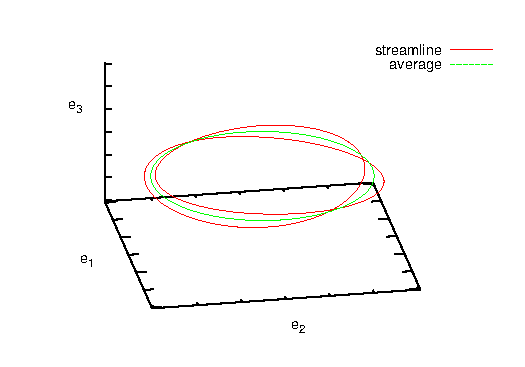
\includegraphics{trefoil_knot.pdf}
 \caption{
   A possible streamline (red) with its averaged rotation in green.
   The streamline was chosen to be a trefoil knot. The reasons for the non-trivial topology are discussed in the text.
   }
   \label{fig:particle}
\end{figure}

\subsection{Interactions between spinless charges}\label{sec:spinless}
When an acoustic charge has no spin (or the spin is ignored)
the equations of motion can be derived from the manifestly gauge invariant energy momentum tensor in  \eqnref{TAEM}.
By taking the  divergence and picking out the spatial terms,
the force $\vf$ is found to be \cite{Doran2003}
\begin{align}
  \vf = - \lr{\rho_q\vE + \vJ \times \vB}.
\end{align}
If it is assumed that an acoustic charge $q$ is carried by a `particle' (a vortex tube without swirl, for instance)
moving at speed $\vu$, then
$\vf = - q\lr{\vE + \vu \times \vB}$, which is the Lorentz force law.
We argue, therefore, that turbulent sources of sound, interact according to the Lorentz-force law when measured acoustically.

The force law takes the form
\eqal{
\dot  u  = - \frac{q}{m_0} F \cdot u
}{LorentzGA}
when expressed with geometric algebra, where the dot denotes differentiation 
with respect to proper time and $m_0$ is the {\em rest mass} of the vortex source,
presumably the mass  displaced by the differing density of the vortex.
% The divergence of the energy momentum tensor gives the force
% and the spatial component in the lab frame is
% \begin{align}
%   \vf = - \lr{\rho_q\vE + \vJ \times \vB}.
% \end{align}
% If it is assumed that an acoustic charge $q$ is carried by a `particle' moving at speed $\vu$, then
% $\vf = - q\lr{\vE + \vu \times \vB}$, which is the Lorentz force law.
% Turbulent sources of sound, therefore, interact according to the Lorentz-force law when measured acoustically.

%\subsection{Particles with Spin}

\subsection{Interactions between particles with spin}\label{sec:spin}
Vortex rings with swirl,
by virtue of their angular momentum about their symmetry axis, have been used as  classical models of spin \cite{Pekeris1953}.
It is, however, the link between topology, helicity and spin that makes the analogy more than a useful conceptual aid.
Moffatt \cite{Moffatt1969}, for example, when considering Hicks' spherical vortex notes  that 
``every torus knot is represented once and only once amongst all the vortex lines of each member of the family of flows described by the stream function''.
Accordingly, the intrinsic angular momentum of such toroids 
can be at least partially identified with its spin.
%The spin will interact with an external vorticity field with a magnetic moment type reaction.
%By appeal to the electromagnetic analogy we call the strength of the interaction the {\em magnetic moment}.
%Since there is no danger of confusion, it seems better to use the terms of the analogy rather than introducing names such as {\em vorticity-moment}.
%The magnetic moment is $\mu = \gamma_g \vs$ where $\vs$ is the spin vector and $\gamma_g$ is the giromagnetic ratio.
%The energy of the interaction is $H = \mu \cdot \vB$. % and accordingly the force is $-\vdel H =-\vdel  \mu\cdot \vB$.
%The spin-vorticity interactions need to be added
%to the Lorentz force law of \eqnref{LorentzGA}.


The kinematics of a vortex ring can be modelled by placing a local orthonormal coordinate frame $\{e_0, e_1, e_2, e_3\}$ at the centre of the ring.
The vector $e_0$ is timelike and is tangent to spacetime path of the centre of the vortex, $x(\tau)$.
Then, with $\tau$ being the proper time, $e_0 = \frac{dx}{d\tau} = u$, where $u$ is the velocity, and $e_0^2 = 1$.
The three orthogonal axes are spacelike, so that $e_i^2 = -1,$ for $i = 1,2,3$.
The vector $e_3 = s$ is oriented so that it is  orthogonal to the vortex ring, and is called the spin vector.
The vectors, $e_2$ and $e_1$ define the {\em spin-plain}, $S = e_2e_1$ on which the vortex ring is confined.
The vector $e_2$ is set to point towards the average motion of a particular swirling particle (following the green line in  \figref{particle})
enabling the magnitude of the spin to be captured.

%If the vortex is moving inertially, its momentum $p$ will be constant.
%%$m$ is a measure of the vortex's intrinsic mass, perhaps the mass difference displaced by any pressure gradients within the vortex.
%By defining and effective mass, $m =  p \cdot u$ and integrating, it follows that  $p\cdot(z - z_0) = m\tau$.
%If the angular momentum is conserved then $lr{z - z_0} \wedge p = S(\tau) - S_0$ and so the equation of motion follows
%\begin{align}
%z = (S(\tau) - S_0) \cdot p^{-1} + m p^{-1} \tau + z_0 = x(\tau) + r(\tau),
%\end{align}
%where $x(\tau) = S_0 \cdot p^{-1} + m p^{-1} \tau + z_0 $ is the spacetime path of the central line, 
%and $r(\tau) = S(\tau)  \cdot p^{-1}$ is the radius of the vortex ring.
%The particle that is followed by $e_2$ is then seen to follow a helix of radius $r$ in spacetime.
Although it is not immediately obvious,
the model presented so far is essentially identical to the `timelike' case of the David Hestenes zitterbewegung interpretation of 
electron physics 
\cite{Hestenes1973, Hestenes1990,  HestenesResearchProgram}. 
We apply the results of these papers freely, 
although argue the results in terms of the meaning to acoustically measured turbulence. 


The motion of the reference frame $\{e_\mu\}$ models the motion of the vortex
and can be obtained from a constant reference frame, $\{\gamma_\mu\}$ by means a Lorentz rotation.
Rotations are double sided transformations in geometric algebra, 
and is written,
$e_\mu = R \gamma_\mu \Rt$,
where the {\em rotor} $R$ is an even multivector with reverse $\Rt$, such that $ R\Rt = 1$.
Since geometric positioning of $\{e_\mu\}$ is all that is modelled,
the kinematics of the frame can be completely determined by finding the
$\tau$-dependent bivector $\Omega =  2\dot{R}\Rt $, which represents the angular
velocity of the frame,
%kinematics is expressed entirely by the rotor $R$,
%such that
%\eqal{
%\dot{R} = \half\Omega R.
%}{RotorEqn}
%Alternatively, the influence on each axi
\begin{align}
  \dot e_\mu = \Omega \cdot e_\mu
\end{align}
The Lorentz force in \eqnref{LorentzGA} is of this type, with $\OmegaEM = \frac{q}{m_0}F$.
%where $\Omega =  2\dot{R}\Rt $ is an 
%The dynamics of the frame can be completely determined by finding the
%$\tau$-dependent bivector $\Omega =  2\dot{R}\Rt $, which represents the angular
%velocity of the frame.

The energy of the fluid in the vortex is modelled by the rotation of $e_2$ in the spin plain $S$.
Therefore, energy-momentum of the vortex is described by the rotation in this plain, $\Omega \cdot S$.
%The quantisation of the spin in \secref{lagrangian} came from the knottedness of the flow around the spin-plain, 
%which implies that $\oint \lr{ dx^\mu \Omega_\mu} \cdot S = nk$,
%where $k$ is the vortex strength and $\Omega_\mu$ is the acceleration in the direction of $\gamma_\mu$.
To include interactions with sound wave, 
%If the vortex interacts with sound then for the angular momentum to be both conserved and obey the quantisation,
it should be the  {\em canonical energy-momentum}, $P = p - eA$, that is equated to $\Omega \cdot S$.
%It is appropriate that the sound contributes its energy to the spin, 
%for this is the only way in which angular momentum is conserved. 
Therefore
\begin{align}
  \Omega\cdot S = P \cdot u = m - eA\cdot v.
\end{align}
If a sound wave deposits $\OmegaEM \cdot S$ of energy to the vortex ring, then its mass must also increase.
%The  $m = p \cdot u$ cannot therefore be equal to the free vortex mass $m_0$,
%but must be
Therefore
\begin{align}
  m  = p \cdot u =  \Omega \cdot S + eA\cdot v= m_0 + \OmegaEM \cdot S + eA\cdot v.
\end{align}
The other components of the angular velocity in the direction orthogonal to the spin plain is labelled $ v\cdot  ( I q) =- v\cdot (\Omega \wedge S)$
while the rate at which the spin plain changes direction as it moves round its axis is $\dot S = v \cdot \del S = \Omega \times S$.
Note that the symbol $\times$ here represents the commutator product rather than the Gibbs vector product.
Bringing all the components together
\begin{align}
\label{eqn:OmegaS}
\Omega S = \Omega \cdot S + \Omega \times S + \Omega \wedge S  = v \cdot P + \dot S + Iq
\end{align}

An explicit expression for $\Omega$ can be obtained by setting
\begin{align}
  \label{eqn:OmegaS2}
  \Omega S &= m_0 + \OmegaEM S && \implies & \Omega &= m_0 S^{-1} + \OmegaEM = m_0 S^{-1} + \frac{e}{m_0} F.
\end{align}
Clearly then \eqnref{LorentzGA} is satisfied.
Also it follows that  $\dot S = \frac{e}{m_0} F \times S$ which gives an expression for the precession of the spin plain due to the magnetic moment.

Combining \eqnref{OmegaS} and \eqnref{OmegaS2} gives
\begin{align}
   v \cdot p- eA\cdot v  + v \cdot \del  S - v\cdot  (I q)=m_0 + \frac{e}{m_0} F S = m - eA\cdot v 
\end{align}
This is the classical approximation  of the Dirac equation in the absence of statistical terms \cite{Hestenes1990}.
The full  equation in the absence of statistical terms is 
\begin{align}
 p -Iq +  = mv - \del S.
\end{align}
The similarities and differences  between these equations is found in the literature \cite{Hestenes1990}.

\section{Modelling an oscillating Bubble}\label{sec:bubble}
%Micron-sized bubbles are resonant at medical ultrasound frequencies and are used as contrast agents
%for they  greatly enhance the signal  from blood which is generally echo-poor.
%To consider their acoustic output it is often sufficient to ignore turbulence and simply calculate the oscillations of a monopole source.
%However, their {\em motion} will generally not be free from turbulence effect - indeed, the microbubbles are often used to {\em measure} such turbulence.
%It would be nice to bring their interactions with sound into the general framework presented so far.
%To do so, the bubble is assumed to be an enclosed vortex. 
%Toroidal bubbles bound in a region of vorticity have been observed many times - and even generated by Dolphin's in play \cite{}.
%A spherical vortex with swirl is stable even when stationary in the fluid - and it is this flow that we imagine within a bubble.
%In the model presented, the mass of the vortex increases when it absorbs a sound wave.
%This models the volume fluctuations only at their most crude,
%although for the purpose of dynamics this may be sufficient.


To adequately model the dynamics of pulsating body such as a bubble, the  {\em interaction parameter}, $\beta$  needs to be introduced into the model.
This can be done by substituting  $F \rightarrow F e^{I\beta}$ in the model above.
Since the bubbles are very small, we additionally introduce a probability density $\rho$ for their location 
- where the symbol $\rho$ should not be confused with the mass or charge density.
Inserting these into the model above results in
\begin{align}
   \rho v \cdot p e^{-I\beta}  + v \cdot \del  \lr{\rho S e^{I\beta}} - \rho v\cdot  (I q)= \rho m \cos\lr{\beta}
\end{align}
This is the classical limit to the full Dirac equation including `statistical factors' \cite{Hestenes1973}
The interaction intensity $\beta$ is uninterpreted in Dirac theory, although it is known to be important for determining whether an election is in a particle or anti-particle state.
Here $\beta$ plays a similar role (it determines whether the force is attractive or repulsive).
Whether the identification stands up to scrutiny remains to be seen.

\section{Discussion}\label{sec:discussion}

We have constructed a general model for the dynamic interactions between sound, turbulence and bubbles.
If the model is confirmed experimentally,
then it represent a  relatively simple yet powerful framework in which to investigate the motion and dynamics of acoustic sources.

In order to be able to construct the models the following observations were necessary:
\nlist{
\item  That the measurement process used in acoustical measurement is identical to that used in optical relativistic theories,
    but with the speed of sound taking the role of the speed of light.
\item  That acoustics formulated on an incompressible, relativistic ideal fluid (which embodies measurement considerations)
    is identical to classical electromagnetism.
}
The authors are unaware of these observations having been made before.

Having made the link between electromagnetism and acoustics, 
for which a relativistic theory is  a pre-requisite,
the application to acoustic interactions followed more-or-less mechanically.
This indicates, on the one hand, the potential power of the analogy.
It represents, on the other hand, a set of stringent experimental test with which to test the link between acoustics, relativity and electromagnetism.


%%% Local Variables: 
%%% mode: latex
%%% TeX-master: "../../tshorrock_thesis"
%%% End: 
